\documentclass{letter}
  \usepackage{tikz}
   \def\firstcircle{(0,0) circle (3cm)}
  \def\secondcircle{(3,0) circle (3cm)}
  \def\thirdcircle{(1.5,3) circle (3cm)}
  %\def\firstcircle{(90:1.75cm) circle (2.5cm)}
  %\def\secondcircle{(210:1.75cm) circle (2.5cm)}
  %\def\thirdcircle{(330:1.75cm) circle (2.5cm)}
  \def\boundingbox{(-3,-3) rectangle (6,4.5)}
  \begin{document}
    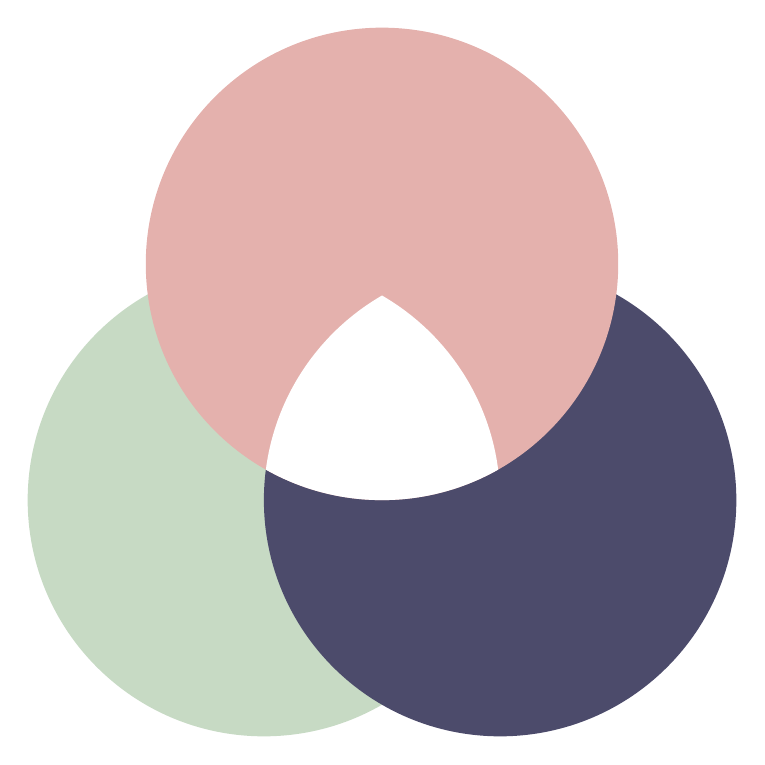
\begin{tikzpicture}
    \definecolor{Lin}{HTML}{C7DAC4}
    \definecolor{Psy}{HTML}{4C4B6B}
    \definecolor{CS}{HTML}{E4B1AD}
    \definecolor{IN}{HTML}{C8CADF}
      \begin{scope}
    %\clip \secondcircle \thirdcircle
    \fill[Lin] \firstcircle node[xshift=-1.5cm, yshift=-.5cm] {Linguistics};;
    \fill[Psy] \secondcircle node[xshift=1.5cm, yshift=-.5cm] {Psychology}; ;
    \fill[CS]  \thirdcircle node[yshift=1cm] {Comupter Science};;
      \end{scope}
      
       
	  \begin{scope}
	 \clip \firstcircle;
	 \clip \secondcircle;
	 \fill[white] \thirdcircle;
	 \end{scope}
  
     
      
    \end{tikzpicture}
  \end{document}